%!TEX root = /Users/rafaeldurelli/Dropbox/Artigos Elaborados/KDM propagation_2015/sbes_2015_kdm_propagation/sbes2015_kdm_propagation.tex

\section{Background} % (fold)
\label{sec:background}

In this section we provide a brief background to Architecture-Driven Modernization (ADM) and Knowledge Discovery Metamodel (KDM). 

%Further, we describe in detail why change propagation in KDM is a complex process.

\subsection{ADM and KDM}

The growing interest in using Model-Driven Development (MDD) to manage software evolution~\cite{Heckel2008, Andrade:2005, Reus:2006} 
%
%
%is mainly focused on the reengineering or modernization of legacy systems. Several software migration projects have been carried out with model-driven approaches~\cite{Heckel2008, Andrade:2005, Reus:2006}. %In addition, the 
%This interest 
motived OMG to define the ADM initiative~\cite{1686216} which advocates carrying out the reengineering process considering MDD principles. 

ADM is the concept of modernizing existing systems with a focus on all aspects of the current systems architecture and the ability to transform current architectures to target architectures by using all principles of MDD~\cite[p.~60]{Ulrich:2010:IST:1841736}. 


Figure~\ref{fig:ADM_shorseshoe} depicts the horseshoe model (i.e., horseshoe is basically a left-hand
side, a right-hand side and a bridge between the sides) which was adapted to ADM. %Please note that it contains all the traditional phases and some MDD's keywords, such as PSM and  PIM. The traditional phases adapted to ADM are:
As can be seen, this horseshoe model contains three main phases:

\begin{itemize}

\item \textbf{Reverse Engineering}: it takes a legacy system to be modernized as input, then the knowledge is extracted and a Platform-Specific Model (PSM) is generated. In addition the PSM serves as the basis for the generation of a Platform-Independent Language (PIM), which is called KDM;

\item \textbf{Restructuring}: in this phase a set of restructuring/refactoring can be applied into a model's instance by means of model transformations;

\item \textbf{Forward Engineering}: then a forward engineering is carried out and the source code of the modernized target system is generated.

\end{itemize} 

%Figure~\ref{horseshoe} depicts the ADM modernization domain model where the left side of the horseshoe is the current state of a busines/it architecture ``as is'' and the right side is what we want to get after the modernization ``to-be''. %One common path followed by IT is to focus on the technical architecture. Generally, the cost of this approach is lower and project duration shorter because the data and application architectures remain largely intact but there is almost no impact or value to the business. 

%On the other hand, a modernization which seeks to provide value to the business, would need to change the application and data architecture, which in turn would rely on an analysis of requirements stemming from shifts to the business architecture. These types of projects are of a longer duration, require more investment, and deliver significantly more value to the business.


\begin{figure}[!ht]
\centering
  % Requires \usepackage{graphicx}
 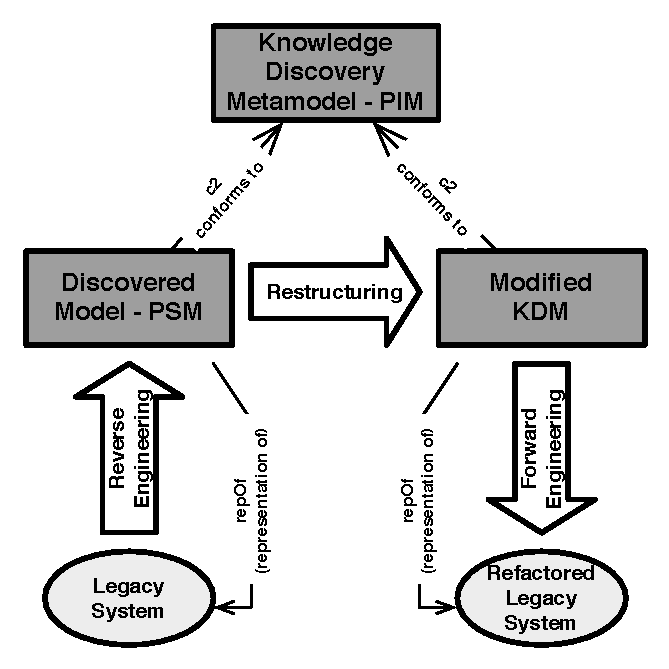
\includegraphics[scale=0.55]{figuras/horseshoes}
\caption{Horseshoe Modernization Model. This figure is adapted from~\cite{OMG_ADM}.}
\label{fig:ADM_shorseshoe}
\end{figure}

In order to perform a systematic modernization as depicted in Figure~\ref{fig:ADM_shorseshoe}, ADM introduces several modernization standards, among them there is the Knowledge Discovery Metamodel (KDM).
%However, herein we focus on KDM because it is the key cornerstone of ADM and the main ideas of our research. 
KDM is an OMG specification adopted as ISO/IEC 19506 by the International Standards Organization for representing information related to existing software systems. 
The goal of the KDM standard is to define a metamodel to represent all the different legacy software artifacts involved in a legacy information system (e.g. source code, user interfaces, databases, business rules, etc.). %The metamodel of the KDM standard provides a comprehensive high-level view of the behavior, structure and data of legacy information systems by means of a set of facts. 

KDM contains twelve packages and it is structured in a hierarchy of four layers: (\textit{i}) Infrastructure Layer, (\textit{ii}) Program Elements Layer, (\textit{iii}) Runtime Resource Layer, and (\textit{iv}) Abstractions Layer. These layers can be instantiated automatically, semi-automatically or manually through the application of various techniques of extraction of knowledge, analysis and transformations~\cite{1686216}. Figure~\ref{fig:kdmLayers} depicts the architecture of KDM and its layers. By observing this figure it is fairly evident that each layer is based on the previous layer. They are organized into packages that define a set of metamodel, whose purpose is to represent a specific and independent interest of knowledge related to legacy systems, e.g. source code, user interfaces, databases, business rules, etc.

\begin{figure}[!ht]
\centering
  % Requires \usepackage{graphicx}
 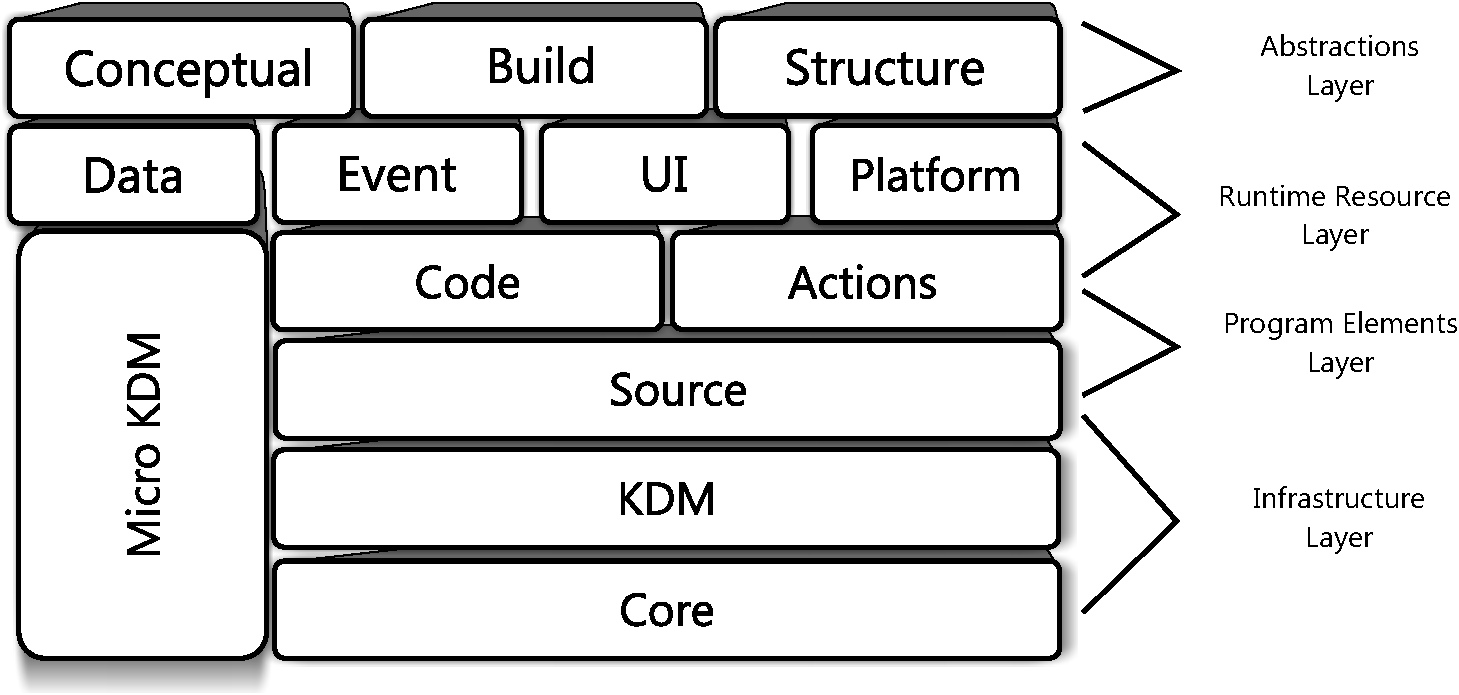
\includegraphics[width=3.3in]{figuras/camadas_kdm}
\caption{KDM Architecture.}
\label{fig:kdmLayers}
\end{figure}

Although KDM is a metamodel to represent a whole system, its main purpose is not the representation of models related strictly to the source code nature such as Unified Modeling Language (UML). While UML can be used to generate new code in a top-down manner, an ADM-based process using KDM starts from the different legacy software artifacts and builds higher-abstraction level models in a bottom-up manner through reverse engineering techniques. %KDM can be seen from different perspectives, as follows: (\textit{i}) KDM can be considered as a metamodel to represent legacy knowledge models, (\textit{ii}) most of the KDM specification is a definition of a language- and platform-independent ontology of legacy information systems and (\textit{iii}) KDM is a common interchange format that makes the interoperability between the reverse engineering tools and modernization tools possible.

%KDM specification owns some KDM domain, each domain defines an architectural viewpoint. In order to define the catalogue of refactoring for the KDM we need to focus just on the Program Element Layer - more specifically  in the Code Package, which represents the code elements of a program (classes, fields and methods) and their associations. %We are interested in the Code Package once our catalogue is based on fine-grained refactorings, i.e., refactorings to be applied into classes, fields and methods. 
%Therefore, it is important to dig a little deeper in the Code Package.
%
%In a given KDM instance, each instance of the code meta-model element represents some programming language construct, determined by the programming language of the existing software system. Each instance of a code meta-model element corresponds to a certain region of the source code in one of the artifacts of the existing software system. In addition, 
%
%The Code Package consists of $24$ classes and contains all the abstract elements for modeling the static structure of the source code. In Table~\ref{tab:mappingCodeToKDM} is depicted some of them. This table identifies KDM metaclasses possessing similar characteristics to the static structure of the source code. Some metaclasses can be direct mapped, such as Class from object-oriented language, which can be easily mapped to the ClassUnit metaclass from KDM.


%\begin{table}[!h]
%\caption{Metaclasses for modeling the static structure of the source-code}
%\label{tab:mappingCodeToKDM}
%\centering
%\begin{tabular}{|>{\centering}p{3cm}|>{\centering}p{3cm}|}
%\hline 
%Source-Code Element & KDM Element\tabularnewline
%\hline 
%\hline 
%Class & ClassUnit\tabularnewline
%\hline 
%Interface & InterfaceUnit\tabularnewline
%\hline 
%Method & MethodUnit\tabularnewline
%\hline 
%Field & StorableUnit\tabularnewline
%\hline 
%Local Variable & Member\tabularnewline
%\hline 
%Parameter & ParameterUnit\tabularnewline
%\hline 
%Association & KDM RelationShip\tabularnewline
%\hline 
%\end{tabular}
%\end{table}

  %\begin{figure}[!ht]
  %\centering
  % Requires \usepackage{graphicx}
    %\includegraphics[scale=0.39]{FIGURAS_DA_REFATORACAO/ProgramLaye0r}
  %\caption{Chunk of the Code Package (OMG Group~\cite{OMGADM})}
  %\label{fig:programLayer}
  %\end{figure}

 %As can be seen in Figure~\ref{fig:programLayer} the root metaclass is \textit{ComputationalObject} which has two sub-metaclasses, i.e., \textit{DataElement} and \textit{ControlElement}. The former sub-metaclass, \textit{DataElement}, is a generic modeling element that defines the common properties of several concrete classes that represent the named data items of existing software systems, for example, global and local variables, record files, and formal parameters. \textit{DataElement} has five sub-metaclasses - \textit{StorableUnit}, \textit{IndexUnit}, \textit{ItemUnit}, \textit{ParameterUnit} and \textit{MemberUnit}. \textit{StorableUnit} is a concrete  sub-metaclass of the \textit{StorableElement} meta-class that represents variables of the existing software system. \textit{IndexUnit} class is a concrete subclass of the \textit{DataElement} class that represents an index of an array datatype. Instances of \textit{ItemUnit} class are endpoints of KDM data relations which describes access to complex datatypes. \textit{ParameterUnit} class is a concrete subclass of the \textit{DataElement} class that represents a formal parameter; for example, a formal parameter of a procedure. \textit{MemberUnit} class is a concrete subclass of the \textit{DataElement} class that represents a member of a class type. Finally, the latter, \textit{ControlElement} is a sub-metaclass that contains two sub-metaclasses - \textit{MethodUnit} and \textit{CallableUnit}. \textit{MethodUnit} element represents member functions owned by a \textit{ClassUnit}, including user-defined operators, constructors and destructors. The \textit{CallableUnit} represents a basic stand-alone element that can be called, such as a procedure or a function. %As can be seen below the dashed line in Figure~\ref{fig:programLayer} there are also the following enumerations: ``\textit{ExportKind}'', ``\textit{StorableKind}'', ``\textit{CallableKind}'', ``\textit{MethodKind}'', which are sets os literals used as properties of the metaclasses.
 

In order to show how KDM and its metaclasses can be used to represent a system, please considerer a toy system, which is depicted in Figure~\ref{fig:system}. Also, note that this system is used throughout this paper as a running example. 

\begin{figure*}
	\centering
	% Requires \usepackage{graphicx}
	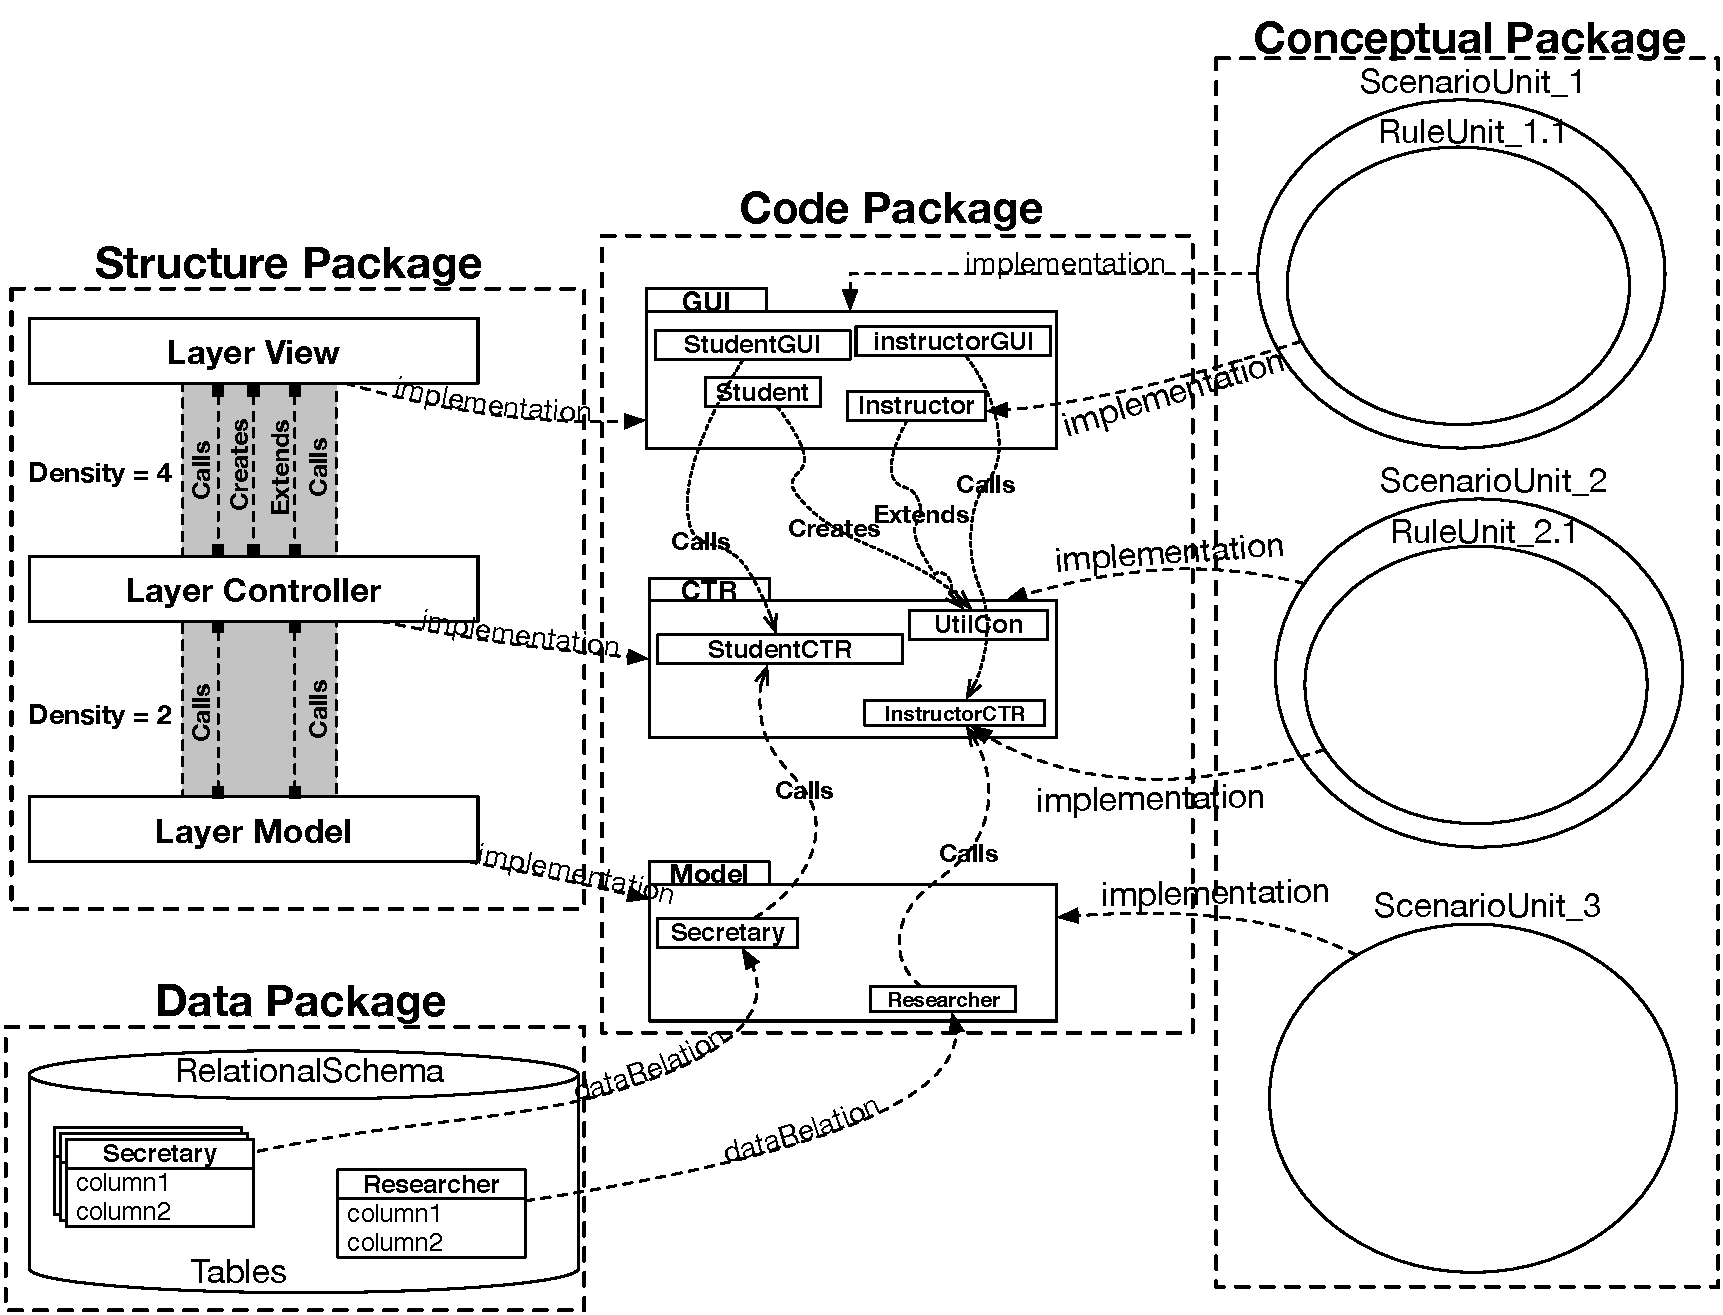
\includegraphics[scale=0.58]{figuras/NewSystemVersion}
	\caption{Motivation and running example.}
	\label{fig:system}
\end{figure*}
 
This toy system is based on a well know Model View Controller (MVC) design pattern. As noted in Figure~\ref{fig:system} it is split in four KDM levels/packages, which are illustrated in the figure bounded by dashed lines shape. %Following is described each KDM levels/packages and its meaning regarding to the illustrated system.

The \texttt{Code Package} represents the source-code (physical artifacts). In Figure~\ref{fig:system} is is possible to see three packages: (\textit{i}) \texttt{GUI} \ding{182}, (\textit{ii}) \texttt{CTR} \ding{183}, and (\textit{iii}) \texttt{Model} \ding{184}. Each of them contains a specific number of classes. %The first one, \texttt{GUI}, contains four classes, \texttt{StudentGUI}, \texttt{InstructorGUI}, \texttt{Student}, and \texttt{Instructor}. The second package contains three classes: \texttt{StudentCTR}, \texttt{UtilCon}, \texttt{InstructorCTR}. Then, the third one owns two classes, \texttt{Secretary} and \texttt{Researcher}. 
Further, these classes are related to each other by means of primitive relationships, such as: \texttt{Calls}, \texttt{Creates}, \texttt{Extends}, etc -  emphasized in Figure~\ref{fig:system} by the symbol \ding{72};

Furthermore, the \texttt{Structure Package} illustrates the system's architecture. As aforementioned the system is based on MVC - each rectangle depicts in Figure~\ref{fig:system} represents a layer, i.e., \texttt{View} \ding{185}, \texttt{Controller} \ding{186}, and \texttt{Model} \ding{186}. %For the first layer, we have associated \texttt{View} with the package \texttt{GUI}. In KDM this kind of association is done by means of the meta-attribute \texttt{implementation}, which are depicted by the dashed arrows. Similarly, \texttt{Controller} was associated with the package \texttt{CTR}, and the layer \texttt{Model} was associated with the package \texttt{Model}, respectively. 
The View layer is realized in source-code level by the package GUI; the Model layer is realized by the package Model and the layer Controller by the CTR package. These realizations are represented in KDM by the \texttt{implementation} relationship, represented in the figure by dashed arrows. Regarding to the relationships among the layers, it is possible to visualize pipes between two layers (see Figure~\ref{fig:system}. These pipes represents the corresponding \texttt{AggregatedRelationship}\footnote{A metaclass in KDM used to represent relationship among KDM entities.}, which represents the number summing all primitive relationships among layers. For instance, the \texttt{AggregatedRelationship} between the layer \texttt{View} and the layer \texttt{Controller} are represented by the relationships: \texttt{Calls}, \texttt{Creates}, \texttt{Extends}, and another \texttt{Calls} from the Code Package. Summing up these relationships the density value is 4. Following the same idea the relationship between the layer \texttt{Controller} and layer \texttt{Model} is 2;  
  
Then the \texttt{Conceptual Package} illustrates the system's business rules domain. Note that this system owns three scenarios, each of them are associated with a package from Code Package by means of the association \texttt{implementation}, see the dashed arrows. Further, each scenario contains a rule except the last one. In it turn, each rule is associated with a class from Code package, again using the association \texttt{implementation};

Finally, the \texttt{Data Package} depicts the system's database and its tables. Herein, it is possible to notice that the depicted system owns a set of Plain Old Java Objects (POJOS), they are: Student, Instructor, Secretary, and Researcher. All of these POJOS are also Object Relational Mapping (ORM), i.e., they are mapped to the Data package using the metaclasse RelationalTable. 

\begin{figure}
	\centering
	% Requires \usepackage{graphicx}
	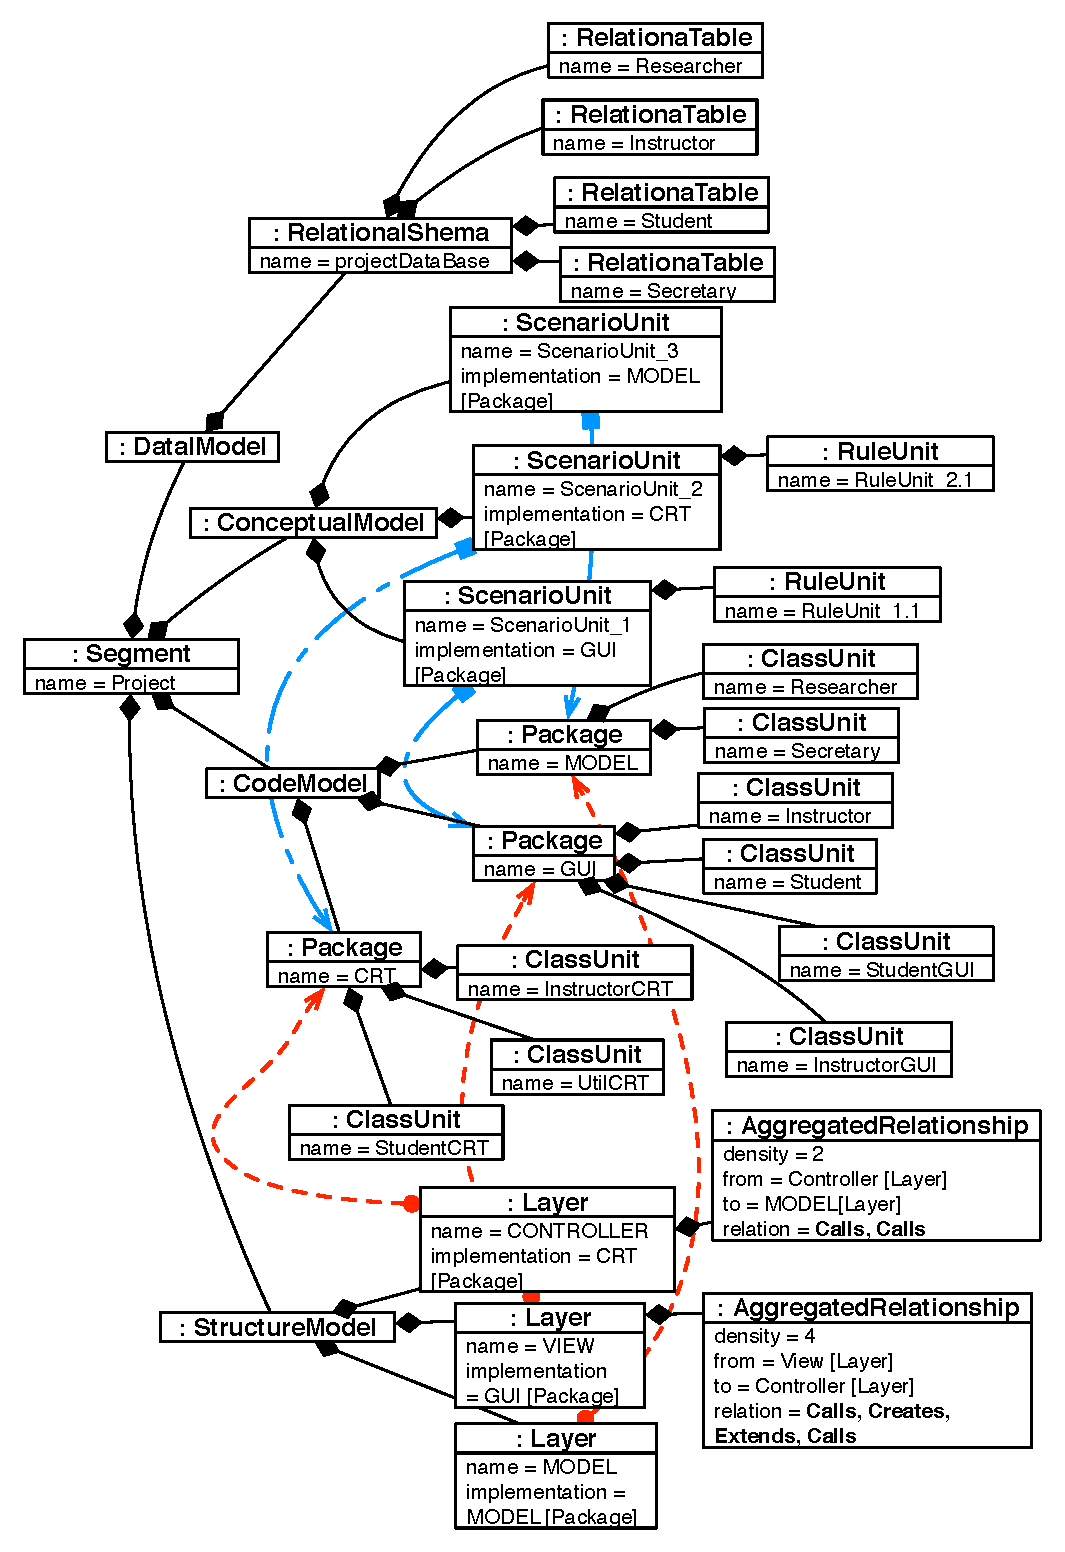
\includegraphics[scale=0.52]{figuras/TreeNewJoint}
	\caption{A bird's eye view of a KDM's instance.}
	\label{fig:allKDMLayers}
\end{figure}

The system described can be realized in KDM as shown in Figure~\ref{fig:allKDMLayers}. This figure depicts the corresponding, though simplified KDM instance of system illustrated in Figure~\ref{fig:system}. We have chosen to use a KDM instance as a UML object diagram for the sake of simplicity. However, it is important to notice that due space limitations some elements are not depicted in this figure.

A KDM's instance can be understood as a tree where we have a specially node called the root of the tree. Then the remaining nodes are partitioned into $\textit{M} >= 0$ joint sets $T_{1}, T_{2}, ..., T_{n}$, and each of these sets is a subtree.  Each nodes represent a metaclass that make up the system depicted in Figure~\ref{fig:system}. The edges represent the relationship between the metaclasses.
%
%
%each KDM's levels/packages can be partitioned both horizontally and vertically; in both cases its metaclasses are closely related and interconnected. %The relations form the key concept of modernization by means of KDM, since they invoke the needs for change propagation. 
%
The root is the metaclass \texttt{Segment}, then, there are four subtrees rooted at \texttt{StructureModel}, \texttt{CodeModel}, \texttt{ConceptualModel}, and \texttt{DataModel}, respectively. 
The tree rooted at \texttt{StructureModel} has three \texttt{Layers}, \texttt{CONTROLLER}, \texttt{VIEW}, and \texttt{MODEL} - they are connected by the metaclasses \texttt{AggregatedRelationship} (see Figure~\ref{fig:system} and Figure~\ref{fig:allKDMLayers}).

The tree rooted at \texttt{CodeModel} has three instance of the metaclass \texttt{Package} - \texttt{CRT}, \texttt{GUI}, and \texttt{MODEL}, respectively. Further, each package contains a set of classes, for instance, the package \texttt{MODEL} has two instance of the metaclass \texttt{ClassUnit}, \texttt{Researcher}, and \texttt{Secretary}, respectively.

The tree rooted at \texttt{ConceptualModel} also has three subtree - herein represented by the metaclass \texttt{ScenarioUnit}. Further, each node of a tree is the root of a \texttt{RuleUnit}. Finally, the \texttt{DataModel} has one subtree - \texttt{RelationalSchema}, which represent the system's data base schema. It contains four subtree - \texttt{Secretary}, \texttt{Researcher}, \texttt{Instructor}, and \texttt{Student}, where each node is an instance of the metaclass \texttt{RelationalTable}.

%(\textit{i}) Code Package, which represents the source-code (physical artefacts), (\textit{ii}) Structure Package, that illustrates the system's architecture, herein the system is based on MVC, (\textit{iii}) Data Package, which depicts the system's database and its tables, and (\textit{iv}) Conceptual Package, which is intended to be the basis for formal and detailed natural language declarative description of a complex entity, such as a business


%owns three layers, they are: (\textit{i}) ``View'', (\textit{ii}) ``Controller'', and (\textit{iii}) ``Model''. Inside of each layer there is at least one package. For instance, the relationships ``GUI inside View'', ``CTR inside Controller'', and ``model inside Model'' mean that ``GUI'', ``CTR'' and ``model'' are contained in ``View'', ``Controller'' and ``Model'', respectively or in some sub-container of  them, transitively. Similarly, the relationship ``StudentGUI inside GUI'' means that ``StudentGUI'' is in container ``GUI'' or in some sub-container of ``GUI''.



%Furthermore, it is possible to notice that the depicted system owns a set of Plain Old Java Objects (POJOS), they are: ``Student'', ``Instructor'', ``Secretary'', and ``Researcher''. All of these POJOS are also Object Relational Mapping (ORM).

\subsection{Model Transformations}\label{sec:m2m}

Kleppe et al.~\cite{Kleppe:2003} provide the following definition of model transformation. \textit{A
transformation is the automatic generation of a target model from a source
model, according to a transformation definition}. 
However, according to Mens and Van~\cite{Mens:2006:TMT:1706639.1706924} model transformations can be classified as either endogenous or exogenous. 

Endogenous transformations are transformations between
models expressed in the same language. Exogenous transformations are
transformations between models expressed using different languages. Further, we can classify the transformation as: (\textit{i}) horizontal, and (\textit{ii}) vertical. A horizontal transformation
is a transformation where the source and target models reside at the same abstraction
level. A typical example is \textit{refactoring}. A vertical transformation is a transformation where the source and target
models reside at different abstraction levels.

\begin{table}[h]
\centering
\caption{Orthogonal dimensions of model transformations.}
\label{tab:orthogonal}
\begin{tabular}{lllll}
\cline{1-3}
\multicolumn{1}{|l|}{Classification} & \multicolumn{1}{l|}{horizontal}                                                 & \multicolumn{1}{l|}{vertical}          &  &  \\ \cline{1-3}
\multicolumn{1}{|l|}{endogenous}     & \multicolumn{1}{l|}{\cellcolor[HTML]{9B9B9B}{\color[HTML]{000000} Refactoring}} & \multicolumn{1}{l|}{Formal refinement} &  &  \\ \cline{1-3}
\multicolumn{1}{|l|}{exogenous}      & \multicolumn{1}{l|}{Language migration}                                         & \multicolumn{1}{l|}{Code generation}   &  &  \\ \cline{1-3}
                                     &                                                                                 &                                        &  & 
\end{tabular}
\end{table}

 Table~\ref{tab:orthogonal} illustrates that the dimensions horizontal versus vertical and endogenous
versus exogenous are truly orthogonal, by giving a concrete example of all
possible combinations. As can be seen in this table our approach focus in endogenous and horizontal transformations.





% models are neither isolated nor static entities. Models are part of an MDA process, and they can be refactored (to improve their internal structure). Refactorings in the context of MDA are implemented as model transformations, i.e., Model-to-Model (M2M). 


%A natural way of implementing refactoring in models is by means of \textit{in-place transformations}, which is illustrated in Figure~\ref{fig:endogenous_inplace}. This kind of transformations are used for rewriting a model by creating, deleting, and updating elements in the input model, e.g., in a KDM's instance. %Going into more details, applying these transformations/refactoring into a KDM's instance can introduce incompatibilities and inconsistencies which can not be easily resolved. In fact, we can classified these transformations by their corrupting or non-corrupting effects~\cite{towardssynchronizing07}:

%\begin{figure}[h]
%	\centering
	% Requires \usepackage{graphicx}
%	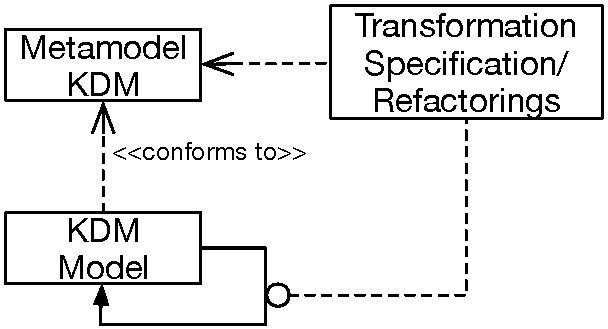
\includegraphics[scale=0.6]{figuras/endogenous_in_place_alg}
%	\caption{Model transformation: in-place.}
%	\label{fig:endogenous_inplace}
%\end{figure} 

